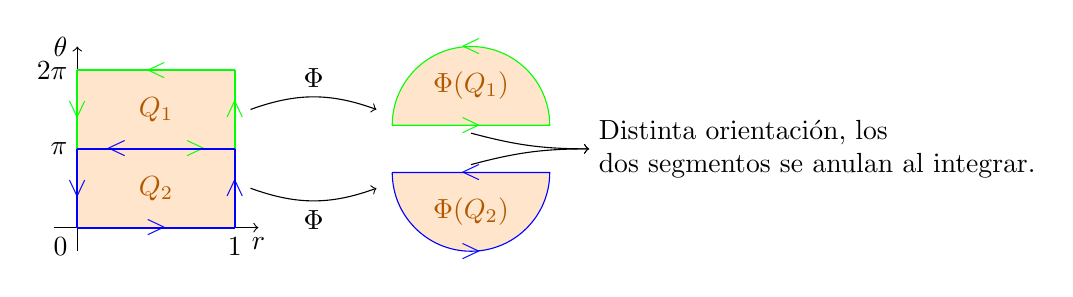
\begin{tikzpicture}
\fill[orange!20!white] (0,0) rectangle (2,2);

\draw[->] (0,-0.3) -- (0,2.3);
\node[left] at (0,2.3) {$\theta$};
\node[left] at (0,2) {$2\pi$};
\node[left] at (0,1) {$\pi$};
\draw[->] (-0.3,0) -- (2.3,0);
\node[below] at (2.3,0) {$r$};
\node[below] at (2,0) {$1$};
\node[below left] at (0,0) {$0$};

\draw[thick,green] (0,1) -- (0,2) node [midway,sloped] {\textless};
\draw[thick,green] (0,2) -- (2,2) node [midway,sloped] {\textless};
\draw[thick,green] (2,2) -- (2,1) node [midway,sloped] {\textless};
\draw[thick,green] (2,1) -- (0,1) node [near start,sloped] {\textgreater};

\draw[thick,blue] (0,0) -- (0,1) node [midway,sloped] {\textless};
\draw[thick,blue] (0,1) -- (2,1) node [near start,sloped] {\textless};
\draw[thick,blue] (2,1) -- (2,0) node [midway,sloped] {\textless};
\draw[thick,blue] (2,0) -- (0,0) node [midway,sloped] {\textgreater};

\node[orange!70!black] at (1,1.5) {$Q_1$};
\node[orange!70!black] at (1,0.5) {$Q_2$};

\draw[->] (2.2,1.5) to[out=20,in=160] node[midway,above,sloped] {$\Phi$} (3.8,1.5);
\draw[->] (2.2,0.5) to[out=-20,in=200] node[midway,below,sloped] {$\Phi$} (3.8,0.5);

\draw[green,fill=orange!20!white] (4,1.3) arc (180:0:1) -- (4,1.3) node[midway] {\textgreater};
\node[green] at (5,2.3) {\textless};
\node[orange!70!black] at (5,1.8) {$\Phi(Q_1)$};


\draw[blue,fill=orange!20!white] (4,0.7) arc (-180:0:1) -- (4,0.7) node[midway] {\textless};
\node[blue] at (5,-0.3) {\textgreater};
\node[orange!70!black] at (5,0.2) {$\Phi(Q_2)$};

\draw[->] (5,1.2) to[out=345, in=180] (6.5,1);
\draw[->] (5,0.8) to[out=15, in=180] (6.5,1);

\node[right,align=left] at (6.5,1) {Distinta orientaci\'{o}n, los\\ dos segmentos se anulan al integrar.};

\end{tikzpicture}